Il nous a été nécessaire de créer des classes métiers représentant fidèlement le comportement réel des tables contenues dans n'importe quel \sgbd

\begin{figure}[!h]
\centering
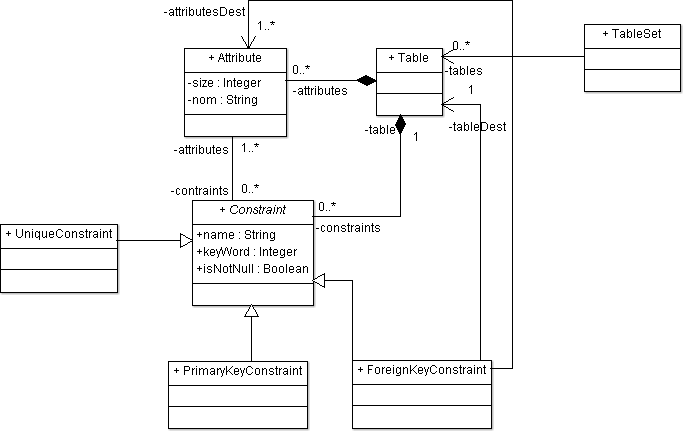
\includegraphics[width=18cm]{images/metier.png}
\caption{Diagramme de classes métiers}
\label{classes_metiers}
\end{figure}


Ces classes ont une particularité, elles peuvent générer du code SQL à partir de leurs attributs ou de différents arguments.
Lorsqu'une table est supprimé, tous les attributs de la table sont détruits et toutes les contraintes composant les attributs et la table sont détruit également.
Si un seul attribut est détruit, toutes les contraintes qui le compose sont détruites, ainsi, une contrainte \textbf{ForeignKeyConstraint} sera détruit même si elle concerne un second attribut.
\exemple{Une fk1 est composé de att1 et att2 pointant sur pk1 et pk2 respectivement.
\newline Si l'on supprime att1, alors la clé étrangère ne peut plus respecter la norme et la contrainte fk1 est détruite.}
